\documentclass[a4paper,11pt]{article}
\usepackage[utf8]{inputenc}
\usepackage{graphicx}
\usepackage{geometry}
\usepackage{hyperref}
\usepackage{booktabs}
\usepackage{listings}
\usepackage{xcolor}
\geometry{margin=1in}

\title{Computer Vision - Mid Project Report}
\author{Alessio Marchetti, Sirio Trentin, Nicolò Spuri}
\date{\today}

\begin{document}

\maketitle

\section{Introduction}
This project implements a system for detecting and localizing moving objects in image sequences. The objective is to output a 2D bounding box representing the coordinates of the detected dynamic object in the first frame of the sequence of images. The solution makes use of techniques to identify and track features over time.

\section{Instructions for Use}
To build and run the project:

\begin{enumerate}
    \item add the images and labels folders in the \texttt{resources} folder, and divided respectively in the \texttt{data} and \texttt{labels} folder;
    \item open the terminal in \texttt{build} path and run \texttt{cmake ..}, \texttt{make};
    \item finally run \texttt{./bin/main} to execute the project;
    \item you can also run \texttt{./bin/main [folder name]} to execute on a specific images folder.
\end{enumerate}

When running the execution command, the program will process all categories in the \texttt{resources/data} folder, compare the generated predictions against the ground truth labels, and automatically generate the results to be viewed in this report.

\section{Approach}
The solution combines traditional computer vision techniques, such as feature extraction (like ORB, SIFT, or KAZE) and optical flow, to differentiate between background motion and dynamic object motion. \\
We started by trying different approaches for the task, in particular: 
\begin{itemize}
    \item Nicolò Spuri tested optical flow with a simple feature detector;
    \item Alessio Marchetti and Sirio Trentin tried to manually track features from one frame to the next, matching feature descriptors.
\end{itemize}
After several tests, we concluded that the best-performing feature detector for this task is SIFT. \\
Then, Alessio Marchetti proposed and implemented a hybrid solution, combining the two previous approaches. A change was made in \texttt{evaluate\_performance.cpp}, where Nicolò Spuri implemented Optical Flow to track features from the current frame to the next. It works as follows:
\begin{enumerate}
    \item every \texttt{hybridApproachRate} iterations, the \texttt{updateTrackedKeypoints} method is called, and \texttt{minMotion} is increased, in order to track only relevant features;
    \item inside the method, the features that survived the previous optical flow iterations are saved in \texttt{verifiedFirstFrameKP};
    \item the current frame's features and descriptors are recomputed;
    \item a matching operation is performed between the initial and current frame descriptors;
    \item the matched features are returned, and optical flow is applied to them.
\end{enumerate}
This serves both to save keypoints after they have survived for some iterations, and to find new keypoints if they were initially stationary.
Finally, Sirio Trentin implemented the testing of the project in \texttt{evaluate\_performance.cpp} and modified the algorithm to dynamically adapt the \texttt{minMotion} distance threshold if the number of keypoints decreases too quickly during the optical flow iterations.\\

\subsection{Workload per member}
\begin{itemize}
    \item Sirio Trentin: 7 hours
    \item Alessio Marchetti: 7.5 hours 
    \item Nicolò Spuri: 8 hours
\end{itemize}

\section{Results}
The project performance on the target dataset (including bird, car, frog, sheep, and squirrel sequences) is evaluated using Mean Intersection over Union (mIoU) and Detection Accuracy (IoU $> 0.5$). 

The automatic results derived from executing the evaluation are included below:

\begin{table}[htbp]
\centering
\begin{minipage}{0.45\textwidth}
\centering
\begin{tabular}{|l|c|}
\hline
\textbf{Category} & \textbf{IoU} \\
\hline
car & 0.7983 \\
sheep & 0.6711 \\
bird & 0.5073 \\
frog & 0.7492 \\
squirrel & 0.0832 \\
\hline
\end{tabular}
\caption{IoU per category.}
\label{tab:iou_per_category}
\end{minipage} \hfill
\begin{minipage}{0.45\textwidth}
\centering
\begin{tabular}{|l|c|}
\hline
\textbf{Metric} & \textbf{Value} \\
\hline
Mean IoU & 0.5618 \\
Accuracy & 0.8000 (4/5) \\
\hline
\end{tabular}
\caption{Overall Performance Metrics.}
\label{tab:overall_metrics}
\end{minipage}
\end{table}

\clearpage
\section*{Initial Frame Tracking Results}
\begin{figure}[htbp]
\centering
\begin{minipage}{0.32\textwidth}
\centering
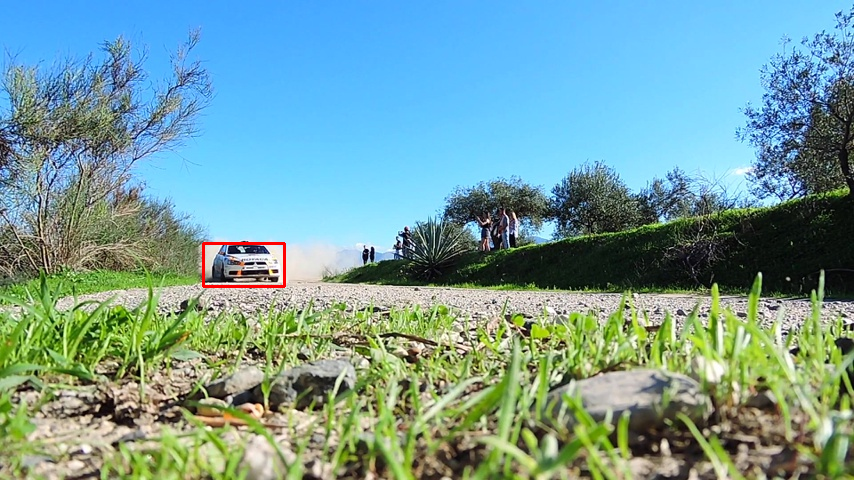
\includegraphics[width=\textwidth]{images/car.png}
\vspace{0.2cm}
\textbf{car}
\end{minipage}\hfill
\begin{minipage}{0.32\textwidth}
\centering
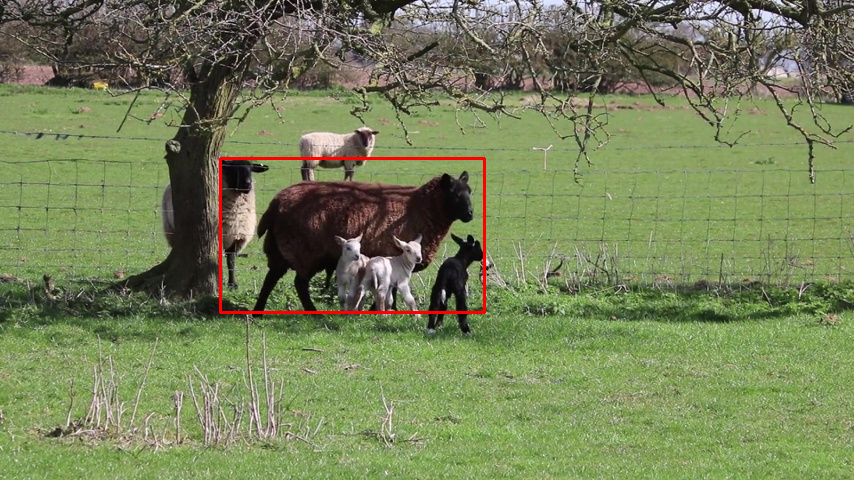
\includegraphics[width=\textwidth]{images/sheep.png}
\vspace{0.2cm}
\textbf{sheep}
\end{minipage}\hfill
\begin{minipage}{0.32\textwidth}
\centering
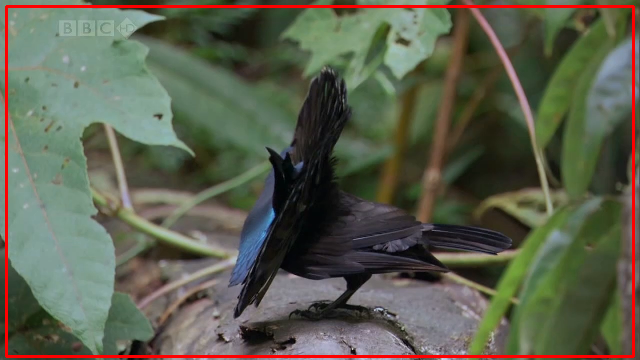
\includegraphics[width=\textwidth]{images/bird.png}
\vspace{0.2cm}
\textbf{bird}
\end{minipage}\hfill
\begin{minipage}{0.32\textwidth}
\centering
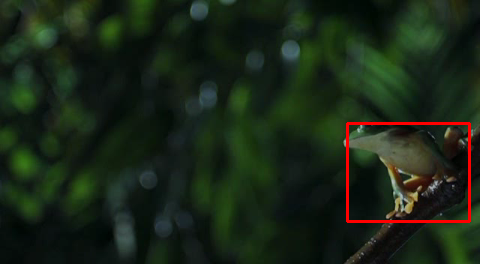
\includegraphics[width=\textwidth]{images/frog.png}
\vspace{0.2cm}
\textbf{frog}
\end{minipage}\hfill
\begin{minipage}{0.32\textwidth}
\centering
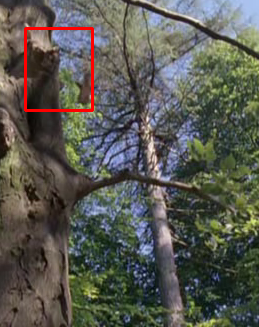
\includegraphics[width=\textwidth]{images/squirrel.png}
\vspace{0.2cm}
\textbf{squirrel}
\end{minipage}\hfill
\caption{Initial Frame for each category with tracked bounding box.}
\end{figure}



\end{document}